\chapter{implementatering}

Ud fra dette og de tilgængelige komponenter på vores komponentalger er vi kommet frem til et print design der ser ud som på figur \ref{printdesign}.

\begin{figure}[H]
	\centering
	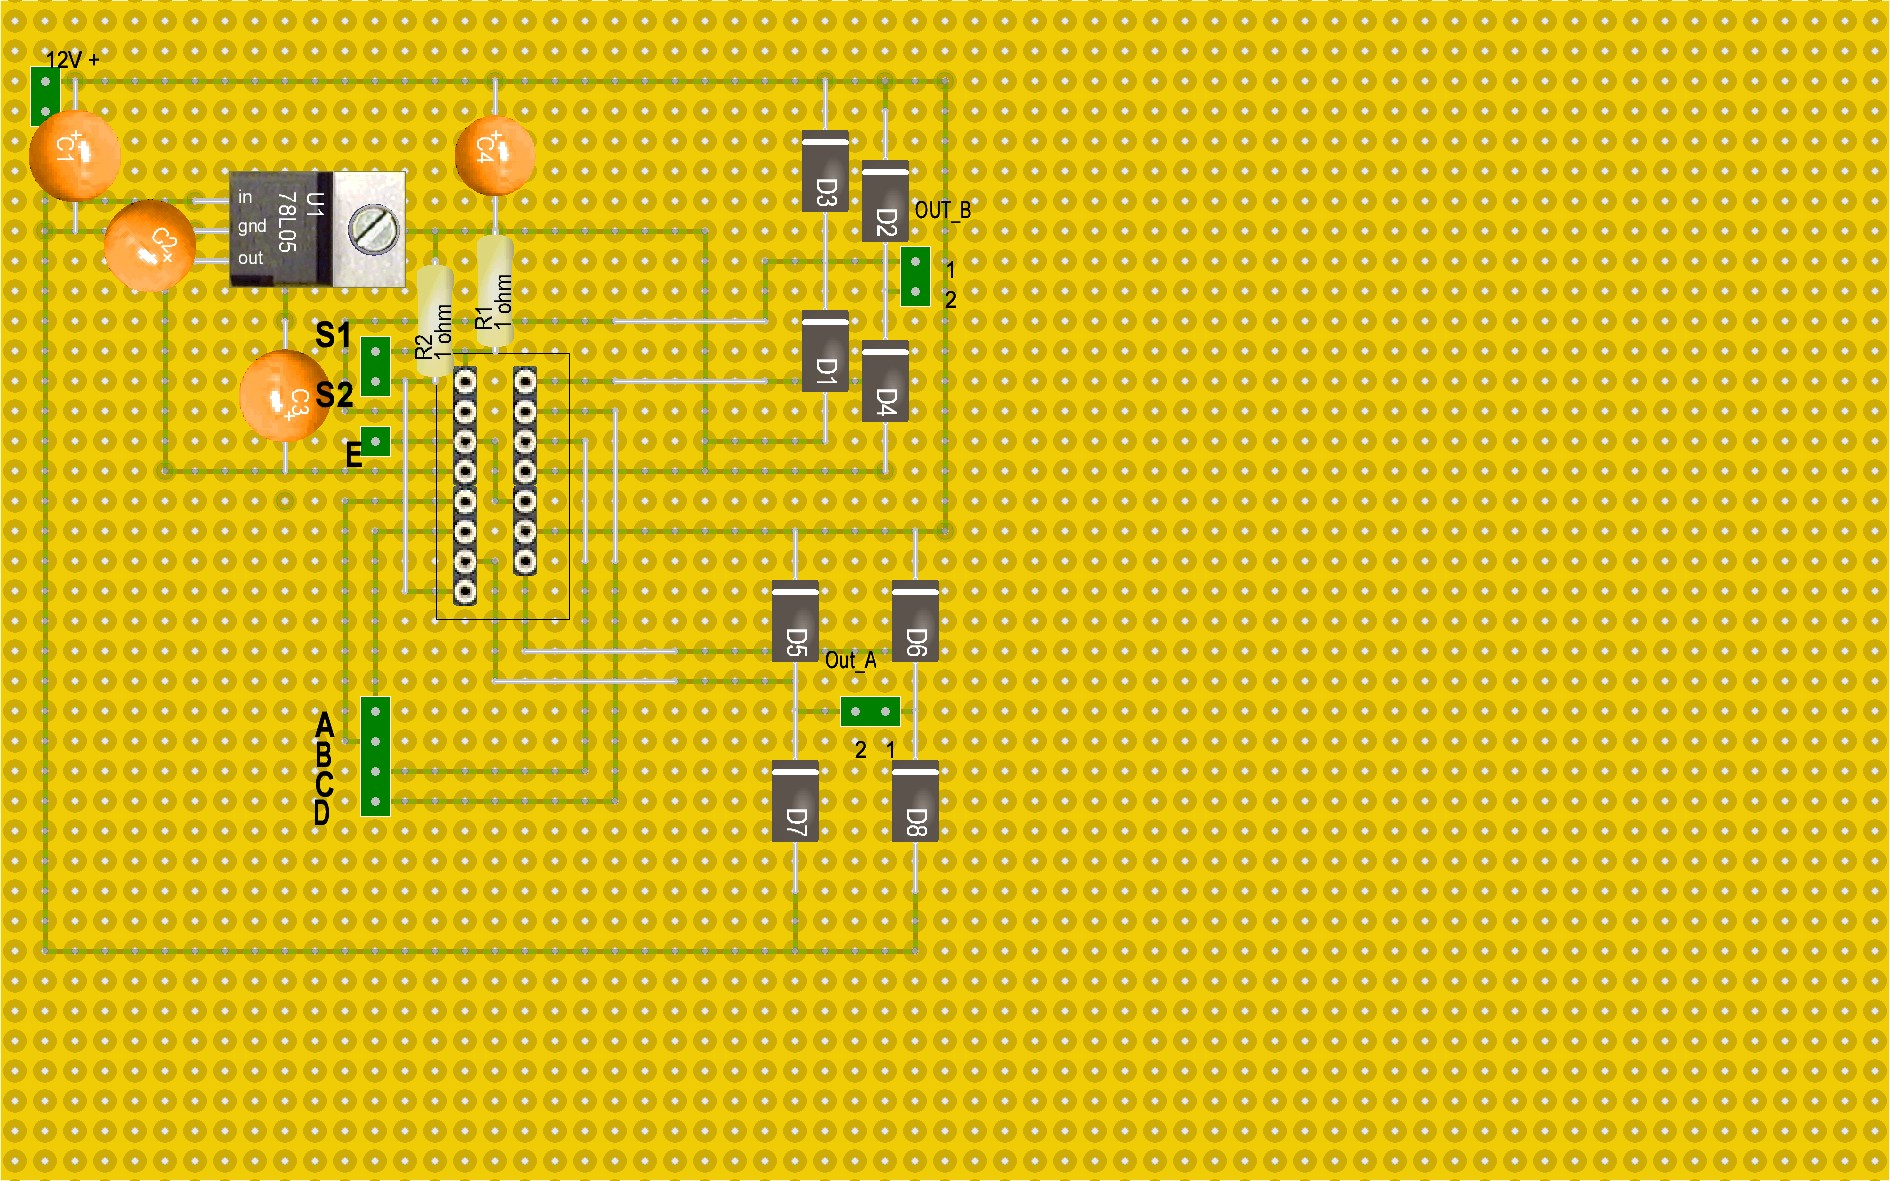
\includegraphics[scale=0.25,trim=0 20 500 0, clip]{billeder/printdesign}
	\caption{Resulterende printdesign}
	\label{printdesign}
\end{figure}

De anvendte dioder er af typen 1N4148 og anvendes som flybackdioder for at beskytte L298 mod de strømme der opstår når spolerne slukkes.

Kondensatorene på det endelig print er ikke af tantalum typen, men værdier er de foreskrevne i databladet for L298.

Det færdige print ses på Figur \ref{solderedprint}.

\begin{figure}[H]
	\centering
	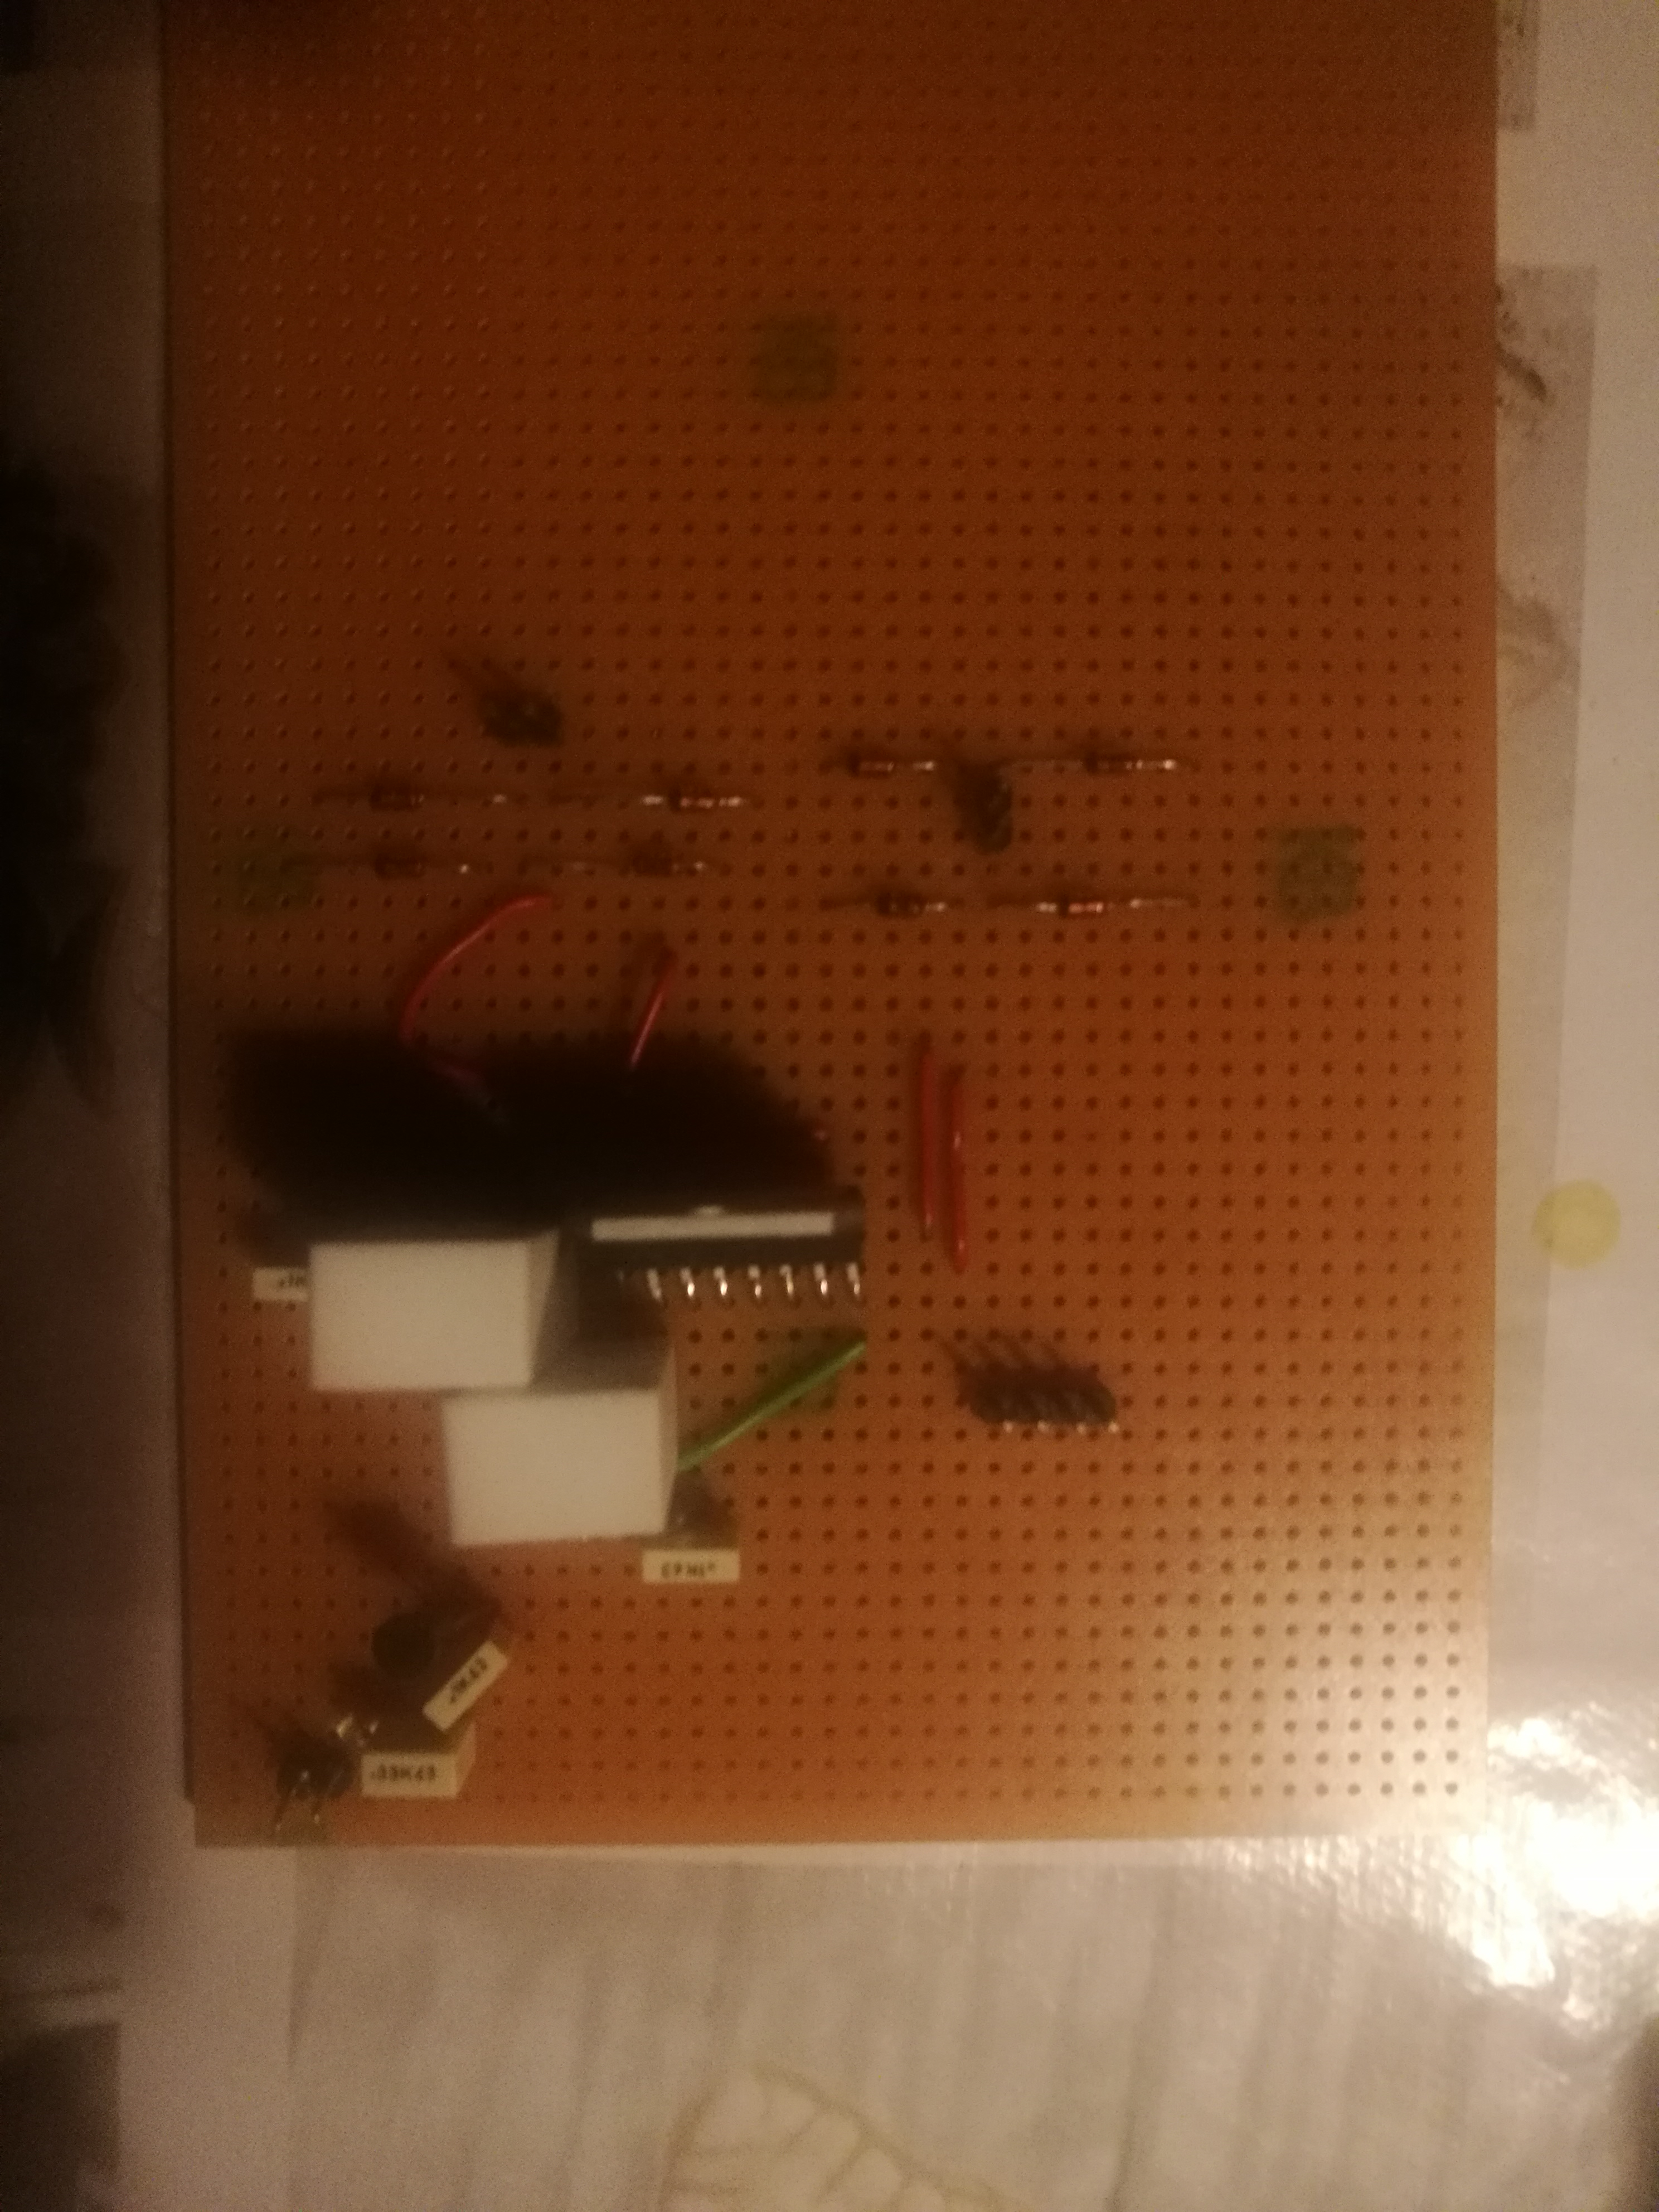
\includegraphics[scale=0.1,trim=0 0 0 0, clip]{billeder/solderedprint.jpg}
	\caption{Resulterende print}
	\label{solderedprint}
\end{figure}
